\documentclass[a4paper,11pt]{article}

% ============================================================
% PACKAGES
% ============================================================
\usepackage[margin=2.2cm]{geometry}
\usepackage{graphicx}
\usepackage{float}
\usepackage{booktabs}
\usepackage{longtable}
\usepackage{array}
\usepackage{xcolor}
\usepackage{hyperref}
\usepackage{enumitem}
\usepackage{amsmath}

\hypersetup{
	colorlinks=true,
	linkcolor=black,
	urlcolor=blue
}

% Disable section numbering for a methodological report style
\setcounter{secnumdepth}{0}

\title{Data Quality Assessment for the Formula 1 Reconciled Database}
\author{Giuseppe Rudi}
\date{\today}

\begin{document}
	
	\maketitle
	
	\tableofcontents
	\newpage
	
	% =======================================================
	\section{Introduction}
	% =======================================================
	
	This document describes the Data Quality Assessment phase applied to the Formula 1 reconciled database.
	The goal of this phase is not to clean the data directly, but to evaluate the current quality level of the data stored in PostgreSQL before applying cleaning rules and before loading the final Data Warehouse.
	
	
	Since the Data Warehouse and the final analytical dashboards depend on the quality of the reconciled level, a systematic assessment is required before continuing with the cleaning and ETL phases.
	
	In this project, Data Quality Assessment is implemented as a deterministic and reproducible Python process that reads the reconciled tables from PostgreSQL, applies a set of quality checks, and produces scorecards and row-level issue files.
	
	% =======================================================
	\subsection{Role of Data Quality Assessment}
	% =======================================================
	
	The Data Quality Assessment phase acts as an audit checkpoint between the reconciled database and the cleaned analytical data.
	Its purpose is to detect data problems before they propagate to the Data Warehouse, the star schema, and the final visual analytics layer.
	
	The project pipeline can be summarized as follows:
	
	\begin{center}
		\begin{tabular}{c}
			Raw and external sources \\
			$\downarrow$ \\
			Extraction and re-engineering \\
			$\downarrow$ \\
			CSV reconciled data \\
			$\downarrow$ \\
			PostgreSQL reconciled database \\
			$\downarrow$ \\
			\textbf{Data Quality Assessment} \\
			$\downarrow$ \\
			Data cleaning \\
			$\downarrow$ \\
			ETL toward the Data Warehouse \\
			$\downarrow$ \\
			Star schema and OLAP analysis
		\end{tabular}
	\end{center}
	

	% =======================================================
	\section{General Data Quality Assessment}
	% =======================================================
	
	It is important to distinguish three different activities: Data Quality Assessment, Data Cleaning, and Analytical Filtering.
	They are related, but they have different goals.
	
	\begin{longtable}{p{3.5cm}p{5.5cm}p{6cm}}
		\toprule
		\textbf{Activity} & \textbf{Goal} & \textbf{Example in this project} \\
		\midrule
		\endfirsthead
		\toprule
		\textbf{Activity} & \textbf{Goal} & \textbf{Example in this project} \\
		\midrule
		\endhead
		Data Quality Assessment & Measure the current quality level and identify problems. & Count missing values in \texttt{lap}, detect duplicate keys, find invalid sector times. \\
		\midrule
		Data Cleaning & Correct, remove, or standardize data quality problems. & Remove deleted or inaccurate laps, standardize textual values. \\
		\midrule
		Analytical Filtering & Select the subset of valid data useful for the final story. & Keep only Ferrari, Red Bull, and Mercedes; keep only dry conditions. \\
		\bottomrule
	\end{longtable}
	

	% =======================================================
	\subsection{Theoretical Background}
	% =========================================================
	
	Data quality is a multidimensional concept.
	For this reason, a single global value is not sufficient to understand whether a dataset is reliable.

	
	The assessment in this project follows the ISO 25012 perspective introduced in the course material.
	The six main dimensions considered are:
	
	\begin{itemize}[leftmargin=1.2cm]
		\item Completeness
		\item Uniqueness
		\item Validity
		\item Consistency
		\item Accuracy
		\item Timeliness
	\end{itemize}
	
	Since this project is based on a relational PostgreSQL reconciled database, an additional practical dimension is also considered:
	
	\begin{itemize}[leftmargin=1.2cm]
		\item Referential Integrity
	\end{itemize}
	
	This additional dimension is essential before adding SQL foreign key constraints and before designing the ETL toward the Data Warehouse.
	
	% ------------------------------------------------------
	\paragraph{Completeness}
	% ------------------------------------------------------
	
	Completeness measures whether required values are present.
	In practical terms, a completeness check verifies the percentage of non-null values for attributes that are necessary to identify, connect, or analyze the records.
	
	In this project, completeness is applied differently depending on the role of each attribute.
	Structural identifiers such as \texttt{lap\_id}, \texttt{session\_id}, \texttt{driver\_id}, and \texttt{team\_id} are expected to be complete.
	Analytical attributes such as \texttt{lap\_time\_ms} may be missing in some special cases and must be evaluated more carefully.
	
	\vspace{2em}
	Formula used conceptually:
	
	\[
	Completeness(A) = \frac{\#\,non\mbox{-}null\ values\ in\ A}{\#\,total\ rows}
	\]
	
	% --------------------------------------------------------
	\paragraph{Uniqueness}
	% --------------------------------------------------------
	
	Uniqueness measures whether keys and candidate keys are free from duplicates.
	This dimension is crucial because the reconciled database must later support primary key constraints and reliable joins.
	
	In this project, uniqueness is checked both on surrogate identifiers and on natural keys.
	For example, \texttt{lap\_id} must be unique if it is used as surrogate key, while the combination \texttt{session\_id + driver\_id + lap\_number} should also identify a lap naturally.
	
	\vspace{2em}
	Formula used conceptually:
	
	\[
	Uniqueness(K) = \frac{\#\,distinct\ key\ values}{\#\,total\ key\ values}
	\]
	
	% --------------------------------------------------------
	\paragraph{Validity}
	% --------------------------------------------------------
	
	Validity measures whether values conform to allowed domains, formats, and business rules.
	A value may be present and unique, but still invalid if it violates the expected domain.
	

	
	% --------------------------------------------------------
	\paragraph{Consistency}
	% --------------------------------------------------------
	
	Consistency measures whether values are coherent with each other.
	This type of check usually compares two or more attributes in the same table, or values stored in different related tables.
	

	% -------------------------------------------------------
	\paragraph{Accuracy and Plausibility}
	% -------------------------------------------------------
	
	Accuracy measures whether values reflect the real-world truth.
	This dimension is difficult to verify automatically without an external reference source.
	For this reason, in this project accuracy is interpreted mainly as plausibility.
	
	A plausibility check does not always prove that a value is wrong.
	Instead, it identifies suspicious values that require further inspection.

	
	% -------------------------------------------------------
	\paragraph{Timeliness}
	% -------------------------------------------------------
	
	Timeliness measures whether data are temporally suitable for their intended use.
	Since this project analyzes historical Formula 1 seasons, timeliness does not mean that the data must be updated to the current day.
	Instead, it means that dates must be coherent with the temporal scope of the analysis.
	

	
	% --------------------------------------------------------
	\paragraph{Referential Integrity}
	% --------------------------------------------------------
	
	Referential Integrity verifies that every foreign key value in a child table points to an existing row in the parent table.


	% =======================================================
	\subsection{Assessment Methodology}
	% =======================================================
	
	The Data Quality Assessment is implemented through a Python script connected to the PostgreSQL reconciled database.
	The script reads the tables, applies deterministic checks, and exports both aggregated scores and detailed issue files.
	
	DA AGGIUNGERE IN FUTURO  => COSA è OUTPUT E COSA SIGNIFICA 
	
	% --------------------------------------------------------
	\subsection{Score Interpretation}
	% --------------------------------------------------------
	
	The scorecard uses a simple interpretation scale:
	
	\begin{longtable}{p{5cm}p{3cm}p{8cm}}
		\toprule
		\textbf{Score Range} & \textbf{Status} & \textbf{Meaning} \\
		\midrule
		\endfirsthead
		\toprule
		\textbf{Score Range} & \textbf{Status} & \textbf{Meaning} \\
		\midrule
		\endhead
		$score \geq 0.95$ & Green & The quality level is acceptable. Only minor monitoring is required. \\
		\midrule
		$0.80 \leq score < 0.95$ & Yellow & The quality level is acceptable for exploration, but cleaning should be planned. \\
		\midrule
		$score < 0.80$ & Red & The quality problem is critical and may block downstream usage. \\
		\bottomrule
	\end{longtable}
	
	% --------------------------------------------------------
	\subsection{Main Output Files}
	% --------------------------------------------------------
	
	The assessment script is expected to produce the following outputs:
	
	\begin{longtable}{p{7cm}p{9cm}}
		\toprule
		\textbf{Output file} & \textbf{Purpose} \\
		\midrule
		\endfirsthead
		\toprule
		\textbf{Output file} & \textbf{Purpose} \\
		\midrule
		\endhead
		\texttt{dq\_scorecard\_all\_tables.csv} & Detailed scorecard with one row for each table, dimension, and check. \\
		\midrule
		\texttt{dq\_scorecard\_by\_table.csv} & Summary score by table, useful to identify the weakest tables. \\
		\midrule
		\texttt{dq\_table\_profiles.csv} & Basic profiling information such as number of rows, number of columns, and missing values. \\
		\midrule
		\texttt{dq\_issues\_lap.csv} & Row-level issues detected in the \texttt{lap} table. \\
		\midrule
		\texttt{dq\_issues\_result.csv} & Row-level issues detected in the \texttt{result} table. \\
		\midrule
		\texttt{dq\_issues\_referential\_integrity.csv} & Broken references between child and parent tables. \\
		\midrule
		\texttt{dq\_scorecard\_for\_llm.json} & Compact JSON version of the scorecard, useful only for generating a natural-language explanation. \\
		\bottomrule
	\end{longtable}
	

	% =======================================================
	\subsection{Table-by-Table Data Quality Plan}
	% =======================================================
	
	This section defines the planned checks for each table of the reconciled database.
	The actual numerical results will be inserted after running the Python assessment script.
	

	\subsubsection{Season Table}

	Although the \texttt{season} table was manually created from domain knowledge and
	contains only two records, it is still included in the Data Quality Assessment.
	The goal is to verify that the manually introduced domain table is complete.
	
	\begin{longtable}{p{3.5cm}p{11cm}}
		\toprule
		\textbf{Dimension} & \textbf{Checks} \\
		\midrule
		\endfirsthead
		
		\toprule
		\textbf{Dimension} & \textbf{Checks} \\
		\midrule
		\endhead
		
		Completeness
		& \texttt{season\_year} must be present because it is the structural identifier of the season \\
		\midrule
		
		Uniqueness
		& \texttt{season\_year} must be unique, since it is the primary key of the table. \\
		\midrule
		
		Validity
		& \texttt{season\_year} must belong to the selected analytical scope, namely \texttt{2021} or \texttt{2022}. If present, \texttt{season\_start\_date} and \texttt{season\_end\_date} must be valid dates, and \texttt{number\_of\_events} must be greater than zero. \\
		\midrule
		
		Consistency
		& If both dates are present, \texttt{season\_start\_date} must be before \texttt{season\_end\_date}. Moreover, the year component of the season dates must be coherent with \texttt{season\_year}. \\
		\midrule
		
		Accuracy
		& Not implemented since the \texttt{season} table is a manually introduced domain table, its accuracy is documented through source provenance during the re-engineering phase. \\
		\midrule
		
		Timeliness
		& Not applicable as a freshness check, because the table represents closed historical seasons. Temporal coherence is already evaluated through validity and consistency checks on \texttt{season\_year} and date attributes. \\
		\bottomrule
	\end{longtable}

	

	\subsubsection{Circuit Table}
	
	It is partly based on domain knowledge and includes derived categorical attributes such as circuit and sector categories.
	
	\begin{longtable}{p{3.5cm}p{11cm}}
		\toprule
		\textbf{Dimension} & \textbf{Checks} \\
		\midrule
		\endfirsthead
		
		\toprule
		\textbf{Dimension} & \textbf{Checks} \\
		\midrule
		\endhead
		
		Completeness
		& \texttt{circuit\_id}, \texttt{global\_circuit\_category},
		\texttt{sector1\_category}, \texttt{sector2\_category}, and
		\texttt{sector3\_category} must be present. These attributes are required
		because they identify the circuit and support the analytical classification used
		in the project. \\
		\midrule
		
		Uniqueness
		& \texttt{circuit\_id} must be unique, since it is the primary key of the table \\
		\midrule
		
		Validity
		& \texttt{global\_circuit\_category} must belong to the allowed global circuit
		domain. \texttt{sector1\_category}, \texttt{sector2\_category}, and
		\texttt{sector3\_category} must belong to the allowed sector category domain. \\
		\midrule
		
		Consistency
		& Textual attributes such as \texttt{circuit\_name}, \texttt{country}, and
		\texttt{location} are checked for empty strings, duplicated variants, and
		inconsistent formatting. A geographical consistency check between
		\texttt{country} and \texttt{location} is not implemented automatically because
		it would require an external geographical reference source. \\
		\midrule
		
		Accuracy/Plausibility
		& Not implemented as a fully automatic check. Their plausibility is documented through the manual
		classification process. \\
		\midrule
		
		Timeliness
		& Not applicable as a freshness check. Possible future circuit layout changes are outside the scope of this
		assessment. \\
		\bottomrule
	\end{longtable}
	
	\textbf{Allowed domains:}
	
	\begin{itemize}[leftmargin=1.2cm]
		\item Global circuit category: \texttt{Street}, \texttt{PowerSensitive},
		\texttt{AeroSensitive}, \texttt{Mixed}
		\item Sector category: \texttt{Power}, \texttt{FastCorners},
		\texttt{SlowCorners}, \texttt{Technical}
	\end{itemize}



	\subsubsection{Driver Table}
	
	The \texttt{driver} table contains stable driver master data obtained from the
	Ergast/Jolpica source through the FastF1 interface. 
	
	\begin{longtable}{p{3.5cm}p{11cm}}
		\toprule
		\textbf{Dimension} & \textbf{Checks} \\
		\midrule
		\endfirsthead
		
		\toprule
		\textbf{Dimension} & \textbf{Checks} \\
		\midrule
		\endhead
		
		Completeness
		& \texttt{driver\_id}, \texttt{abbreviation}, and \texttt{last\_name}
		must be present. These attributes are required to identify and describe each
		driver in the reconciled database and in the later analytical model. \\
		\midrule
		
		Uniqueness
		& \texttt{driver\_id} must be unique, since it is the primary key of the table. \\
		\midrule
		
		Validity
		& If present, \texttt{date\_of\_birth} must be a valid date and
		\texttt{driver\_url} must have a valid URL format. If present,
		\texttt{permanent\_number} must be a positive numeric value.
		\texttt{abbreviation} must follow the expected driver-code format, namely
		a short uppercase alphabetic code. \\
		\midrule
		
		Consistency
		& Textual attributes such as \texttt{first\_name}, \texttt{last\_name},
		\texttt{nationality}, and \texttt{abbreviation} are checked for empty
		strings and inconsistent formatting.  \\
		\midrule
		
		Accuracy/Plausibility
		& Not implemented as a fully automatic truth check.  Plausibility can be assessed by flagging
		abnormal values, such as implausible driver ages during the selected
		2021--2022 seasons. \\
		\midrule
		
		Timeliness
		& Not applicable as a freshness check.  \\
		\bottomrule
	\end{longtable}

	\subsubsection{Team Table}
	
	The \texttt{team} table contains constructor/team master data obtained from the
	Ergast/Jolpica source through the FastF1 interface. It is used as a reference table
	to identify teams in results and lap-level data.
	
	\begin{longtable}{p{3.5cm}p{11cm}}
		\toprule
		\textbf{Dimension} & \textbf{Checks} \\
		\midrule
		\endfirsthead
		
		\toprule
		\textbf{Dimension} & \textbf{Checks} \\
		\midrule
		\endhead
		
		Completeness
		& \texttt{team\_id} and \texttt{team\_name} must be present. 
		\texttt{team\_id} is required because it is the structural identifier used
		in joins, while \texttt{team\_name} is required as the readable business
		label used in reports and visual analyses.  \\
		\midrule
		
		Uniqueness
		& \texttt{team\_id} must be unique, since it is the primary key of the table \\
		\midrule
		
		Validity
		& \texttt{team\_id} must follow the expected identifier format, namely a
		non-empty lowercase textual code. If present, \texttt{team\_url} must have
		a valid URL format. Textual attributes such as \texttt{team\_name} and
		\texttt{nationality} must not be empty strings after trimming. \\
		\midrule
		
		Consistency
		& In the final reconciled
		table, textual attributes are checked for duplicated variants, extra spaces,
		and inconsistent formatting. \\
		\midrule
		
		Accuracy/Plausibility
		& Team names and nationalities can be manually
		verified through source provenance if needed. \\
		\midrule
		
		Timeliness
		& Not applicable as a freshness check.  \\
		\bottomrule
	\end{longtable}



	\subsubsection{Grand Prix Table}
	
	The \texttt{grand\_prix} table represents a Formula 1 Grand Prix event in a
	specific season. Each Grand Prix belongs to one season and is associated with
	one circuit. 
	
	\begin{longtable}{p{3.5cm}p{11cm}}
		\toprule
		\textbf{Dimension} & \textbf{Checks} \\
		\midrule
		\endfirsthead
		
		\toprule
		\textbf{Dimension} & \textbf{Checks} \\
		\midrule
		\endhead
		
		Completeness
		& \texttt{grand\_prix\_id}, \texttt{season\_year},
		\texttt{round\_number}, and \texttt{circuit\_id} must be present.
		These attributes are required to identify the Grand Prix, connect it to the
		corresponding season, and associate it with the circuit where it takes place. \\
		\midrule
		
		Uniqueness
		& \texttt{grand\_prix\_id} must be unique, since it is the surrogate primary
		key of the table. The natural key \texttt{season\_year + round\_number}
		should also be unique, because a round number identifies one Grand Prix
		within a specific season. \\
		\midrule
		
		Validity
		& \texttt{round\_number} must be greater than zero. If present,
		\texttt{event\_date} must be a valid date. If present,
		\texttt{event\_format} must belong to the allowed event format domain,
		such as \texttt{conventional} or \texttt{sprint}. Testing events must not be
		included in the reconciled Grand Prix table. If present,
		\texttt{f1\_api\_support} must be a boolean value. \\
		\midrule
		
		Consistency
		& If \texttt{event\_date} is present, it must be coherent with
		\texttt{season\_year}. Textual attributes such as \texttt{event\_name},
		\texttt{official\_event\_name}, \texttt{country}, and \texttt{location}
		are checked for empty strings, duplicated variants, and inconsistent
		formatting. \\
		\midrule
		
		Accuracy/Plausibility
		& Not implemented as a fully automatic truth check for all event attributes.
		For this table, the main plausibility control concerns the matching between each
		Grand Prix and its circuit. Since \texttt{circuit\_id} is introduced during the
		re-engineering phase by matching \texttt{country} and \texttt{location} with the
		\texttt{circuit} table, the correctness of this association must be validated.
		Rows with missing or ambiguous matches are flagged for manual review. \\
		
		Timeliness
		& Temporal checks are limited to
		the validity and consistency of \texttt{event\_date} with the selected
		2021--2022 project scope. \\
		\midrule
		
		Referential Integrity
		& \texttt{season\_year} must exist in the \texttt{season} table and
		\texttt{circuit\_id} must exist in the \texttt{circuit} table. \\
		\bottomrule
	\end{longtable}
	

	\subsubsection{Session Table}

	
	The \texttt{session} table represents a Qualifying or Race session belonging to a specific Grand Prix.
	Free practice sessions are outside the analytical scope of the project.
	
	\begin{longtable}{p{3.5cm}p{11cm}}
		\toprule
		\textbf{Dimension} & \textbf{Checks} \\
		\midrule
		\endfirsthead
		\toprule
		\textbf{Dimension} & \textbf{Checks} \\
		\midrule
		\endhead
		Completeness & \texttt{session\_id}, \texttt{grand\_prix\_id}, \texttt{session\_type} must be present. \\
		\midrule
		Uniqueness & \texttt{session\_id} must be unique. The natural key \texttt{grand\_prix\_id + session\_type} should also be unique. \\
		\midrule
		Validity & \texttt{session\_type} must be either \texttt{Q} or \texttt{R}. \\
		\midrule
		Consistency & \texttt{session\_date} should be coherent with the corresponding Grand Prix date. \\
		\midrule
		Referential Integrity & \texttt{grand\_prix\_id} must exist in the \texttt{grand\_prix} table. \\
		\bottomrule
	\end{longtable}
	

	\subsubsection{Result Table}


	This table is structurally important because it is used to connect drivers and teams to sessions and also supports the enrichment of lap data.
	
	\begin{longtable}{p{3.5cm}p{11cm}}
		\toprule
		\textbf{Dimension} & \textbf{Checks} \\
		\midrule
		\endfirsthead
		\toprule
		\textbf{Dimension} & \textbf{Checks} \\
		\midrule
		\endhead
		Completeness & \texttt{result\_id}, \texttt{session\_id}, \texttt{driver\_id}, \texttt{team\_id}, and \texttt{position} should be present. \\
		\midrule
		Uniqueness & \texttt{result\_id} must be unique. The natural key \texttt{session\_id + driver\_id} should also be unique. \\
		\midrule
		Validity & \texttt{position} must be greater than zero when present. \texttt{points} must be greater than or equal to zero. \\
		\midrule
		Consistency & \texttt{classified\_position}, \texttt{status}, \texttt{time\_ms}, and \texttt{laps} should be checked for coherent interpretation. \\
		\midrule
		Referential Integrity & \texttt{session\_id}, \texttt{driver\_id}, and \texttt{team\_id} must reference existing rows in \texttt{session}, \texttt{driver}, and \texttt{team}. \\
		\bottomrule
	\end{longtable}
	

	\subsubsection{Lap Table}
	
	Each row represents one lap performed by one driver in one specific session.
	
	\begin{longtable}{p{3.5cm}p{11cm}}
		\toprule
		\textbf{Dimension} & \textbf{Checks} \\
		\midrule
		\endfirsthead
		
		\toprule
		\textbf{Dimension} & \textbf{Checks} \\
		\midrule
		\endhead
		
		Completeness
		& \texttt{lap\_id}, \texttt{session\_id}, \texttt{driver\_id},
		\texttt{team\_id}, and \texttt{lap\_number} must be present because they
		identify the lap and connect it to the driver, team, and session context.
		For analytical completeness, the main performance attributes
		\texttt{lap\_time\_ms}, \texttt{sector1\_time\_ms},
		\texttt{sector2\_time\_ms}, \texttt{sector3\_time\_ms}, and
		\texttt{compound} are also checked, because they are required to compare lap
		and sector performance. \\
		\midrule
		
		Uniqueness
		& \texttt{lap\_id} must be unique, since it is the surrogate primary key of
		the table. The natural key \texttt{session\_id + driver\_id + lap\_number}
		should also be unique, because the same driver cannot have two different
		laps with the same lap number inside the same session. \\
		\midrule
		
		Validity
		& \texttt{lap\_number} must be greater than zero. If present,
		\texttt{lap\_time\_ms} and sector times must be positive values.
		Speed attributes such as \texttt{speed\_i1}, \texttt{speed\_i2},
		\texttt{speed\_fl}, and \texttt{speed\_st} must be positive when present.
		\texttt{stint} and \texttt{tyre\_life} must be non-negative or positive
		according to their domain. \texttt{compound} must belong to the expected tyre
		compound domain, and boolean attributes such as \texttt{fresh\_tyre},
		\texttt{is\_personal\_best}, \texttt{deleted},
		\texttt{fastf1\_generated}, and \texttt{is\_accurate} must contain valid
		boolean values. \\
		\midrule
		
		Consistency
		& For normal timed laps, the sum of
		\texttt{sector1\_time\_ms}, \texttt{sector2\_time\_ms}, and
		\texttt{sector3\_time\_ms} should be coherent with
		\texttt{lap\_time\_ms}, allowing a small tolerance for rounding or source
		precision. Session-time attributes should be coherent with the lap timeline.
		Pit-related attributes must be interpreted consistently: the presence of
		\texttt{pit\_out\_time\_ms} or \texttt{pit\_in\_time\_ms} indicates a
		special lap and may explain missing or abnormal lap and sector times.
		Deleted or inaccurate laps are not automatically removed, but they are flagged for the
		later cleaning phase. \\
		\midrule
		
		Accuracy/Plausibility
		& 
		Plausibility is assessed by flagging suspicious values, such as extremely
		low or high lap times, sector times, and speed values. These values are not
		automatically considered wrong, because Formula 1 laps can be affected by
		pit stops, Safety Car periods, rain, red flags, deleted laps, or other special
		racing situations. \\
		\midrule
		
		Timeliness
		& Temporal quality is evaluated through
		the coherence of relative time attributes such as \texttt{time\_ms},
		\texttt{lap\_start\_time\_ms}, and sector session times within each
		session. If \texttt{lap\_start\_date} is present, it should be coherent with
		the corresponding session or Grand Prix date. \\
		\midrule
		
		Referential Integrity
		& \texttt{session\_id}, \texttt{driver\_id}, and \texttt{team\_id} must
		reference existing rows in the \texttt{session}, \texttt{driver}, and
		\texttt{team} tables. \\
		\bottomrule
	\end{longtable}


	\subsubsection{Weather Table}
	
	Each row represents one weather observation
	associated with a session and identified by a relative session time.
	
	\begin{longtable}{p{3.5cm}p{11cm}}
		\toprule
		\textbf{Dimension} & \textbf{Checks} \\
		\midrule
		\endfirsthead
		
		\toprule
		\textbf{Dimension} & \textbf{Checks} \\
		\midrule
		\endhead
		
		Completeness
		& \texttt{weather\_id}, \texttt{session\_id}, \texttt{time\_ms},
		\texttt{air\_temp}, \texttt{track\_temp}, \texttt{rainfall}, and
		\texttt{wind\_speed} must be present. The first three attributes are required
		to identify each weather observation, connect it to the corresponding session,
		and place it on the session timeline. \\
		\midrule
		
		Uniqueness
		& \texttt{weather\_id} must be unique, since it is the surrogate primary key
		of the table. The natural key \texttt{session\_id + time\_ms} should also be
		unique, because a session should not contain two different weather
		observations with the same timestamp. \\
		\midrule
		
		Validity
		& Numerical weather attributes must belong to plausible physical ranges.
		If present, \texttt{air\_temp} and \texttt{track\_temp} must be plausible
		temperature values, \texttt{humidity} must be between 0 and 100,
		\texttt{pressure} must be positive and within a realistic atmospheric range,
		\texttt{rainfall} must be boolean, \texttt{wind\_direction} must be a valid
		degree value, and \texttt{wind\_speed} must be greater than or equal to zero. \\
		\midrule
		
		Consistency
		& \texttt{time\_ms} represents elapsed time from the beginning of the session,
		therefore it must be non-negative and should progress coherently within each
		\texttt{session\_id}. Weather variables are also checked for internal
		plausibility: for example, \texttt{track\_temp} should be reasonably coherent
		with \texttt{air\_temp}, and combinations such as very low humidity with
		\texttt{rainfall = true} should be flagged as suspicious rather than
		automatically treated as errors. \\
		\midrule
		
		Accuracy/Plausibility
		& Not implemented as a truth check against an external meteorological source. Extreme but possible weather values are flagged for review. \\
		\midrule
		
		Timeliness
		& Not applicable as a freshness check. \\
		\midrule
		
		Referential Integrity
		& \texttt{session\_id} must reference an existing row in the \texttt{session}
		table. \\
		\bottomrule
	\end{longtable}

	\subsubsection{Track Status Table}
	
	The \texttt{track\_status} table contains time-varying track condition messages
	recorded during a specific Formula 1 session. Each row represents a change or
	state of the track at a given elapsed time within the session.
	
	Like the \texttt{weather} table, \texttt{track\_status} is not a direct to-one
	branch of the Lap Performance attribute tree, because a session can have many
	track status records over time. However, it is analytically useful because it can
	be used during ETL to derive lap-level or session-level context attributes.
	
	\begin{longtable}{p{3.5cm}p{11cm}}
		\toprule
		\textbf{Dimension} & \textbf{Checks} \\
		\midrule
		\endfirsthead
		
		\toprule
		\textbf{Dimension} & \textbf{Checks} \\
		\midrule
		\endhead
		
		Completeness
		& \texttt{track\_status\_id}, \texttt{session\_id}, \texttt{time\_ms},
		\texttt{status}, and \texttt{message} must be present. The first three
		attributes are required to identify the record, connect it to a session, and
		place it on the session timeline. The attributes \texttt{status} and
		\texttt{message} are also required because they contain the actual track
		condition information. Without them, the row would not provide useful
		analytical context. \\
		\midrule
		
		Uniqueness
		& \texttt{track\_status\_id} must be unique, since it is the surrogate
		primary key of the table. The natural key \texttt{session\_id + time\_ms}
		should also be checked, because a session should not contain multiple track
		status records with the same timestamp unless this is explicitly justified
		by the source. \\
		\midrule
		
		Validity
		& \texttt{time\_ms} must be greater than or equal to zero.
		\texttt{status} must belong to the documented set of track status codes,
		and \texttt{message} must belong to the documented set of track status
		messages. Both attributes must not be empty strings after trimming. \\
		\midrule
		
		Consistency
		& \texttt{time\_ms} represents elapsed time from the beginning of the
		session, therefore it must progress coherently within each
		\texttt{session\_id}. In addition, \texttt{status} and \texttt{message}
		must be coherent with each other: the same numerical status code should
		always correspond to the same textual message. For example, a status code
		representing clear track conditions should not be associated with a Safety
		Car or Red Flag message. \\
		\midrule
		
		Accuracy/Plausibility
		& Not implemented as a truth check against an external race-control source. Suspicious cases, such as unknown status
		codes, unknown messages, or inconsistent status-message pairs, are flagged
		for review. \\
		\midrule
		
		Timeliness
		& Not applicable as a freshness check. \\
		\midrule
		
		Referential Integrity
		& \texttt{session\_id} must reference an existing row in the
		\texttt{session} table. \\
		\bottomrule
	\end{longtable}
	
	
	\textbf{Expected status-message domain:}
	
	\begin{longtable}{p{3cm}p{5cm}p{6cm}}
		\toprule
		\textbf{Status code} & \textbf{Message} & \textbf{Meaning} \\
		\midrule
		\endfirsthead
		
		\toprule
		\textbf{Status code} & \textbf{Message} & \textbf{Meaning} \\
		\midrule
		\endhead
		
		\texttt{1} & \texttt{AllClear} & Normal track condition. \\
		\midrule
		
		\texttt{2} & \texttt{Yellow} & Yellow flag condition. \\
		\midrule
		
		\texttt{4} & \texttt{SCDeployed} & Safety Car deployed. \\
		\midrule
		
		\texttt{5} & \texttt{Red} & Red flag condition. \\
		\midrule
		
		\texttt{6} & \texttt{VSCDeployed} & Virtual Safety Car deployed. \\
		\midrule
		
		\texttt{7} & \texttt{VSCEnding} & Virtual Safety Car ending phase. \\
		\bottomrule
	\end{longtable}
	

	\subsection{Planned Visual Outputs}

	
	The Python assessment script should also generate visual outputs to summarize the results.
	These figures will be inserted in the final version of the report after running the script.
	
	% ------------------------------------------------------------
	\subsubsection{Overall Data Quality Score by Table}
	% ------------------------------------------------------------
	
	This plot compares the average data quality score of each table.
	It is useful to identify which table requires the most cleaning effort.
	
	\begin{figure}[H]
		\centering
		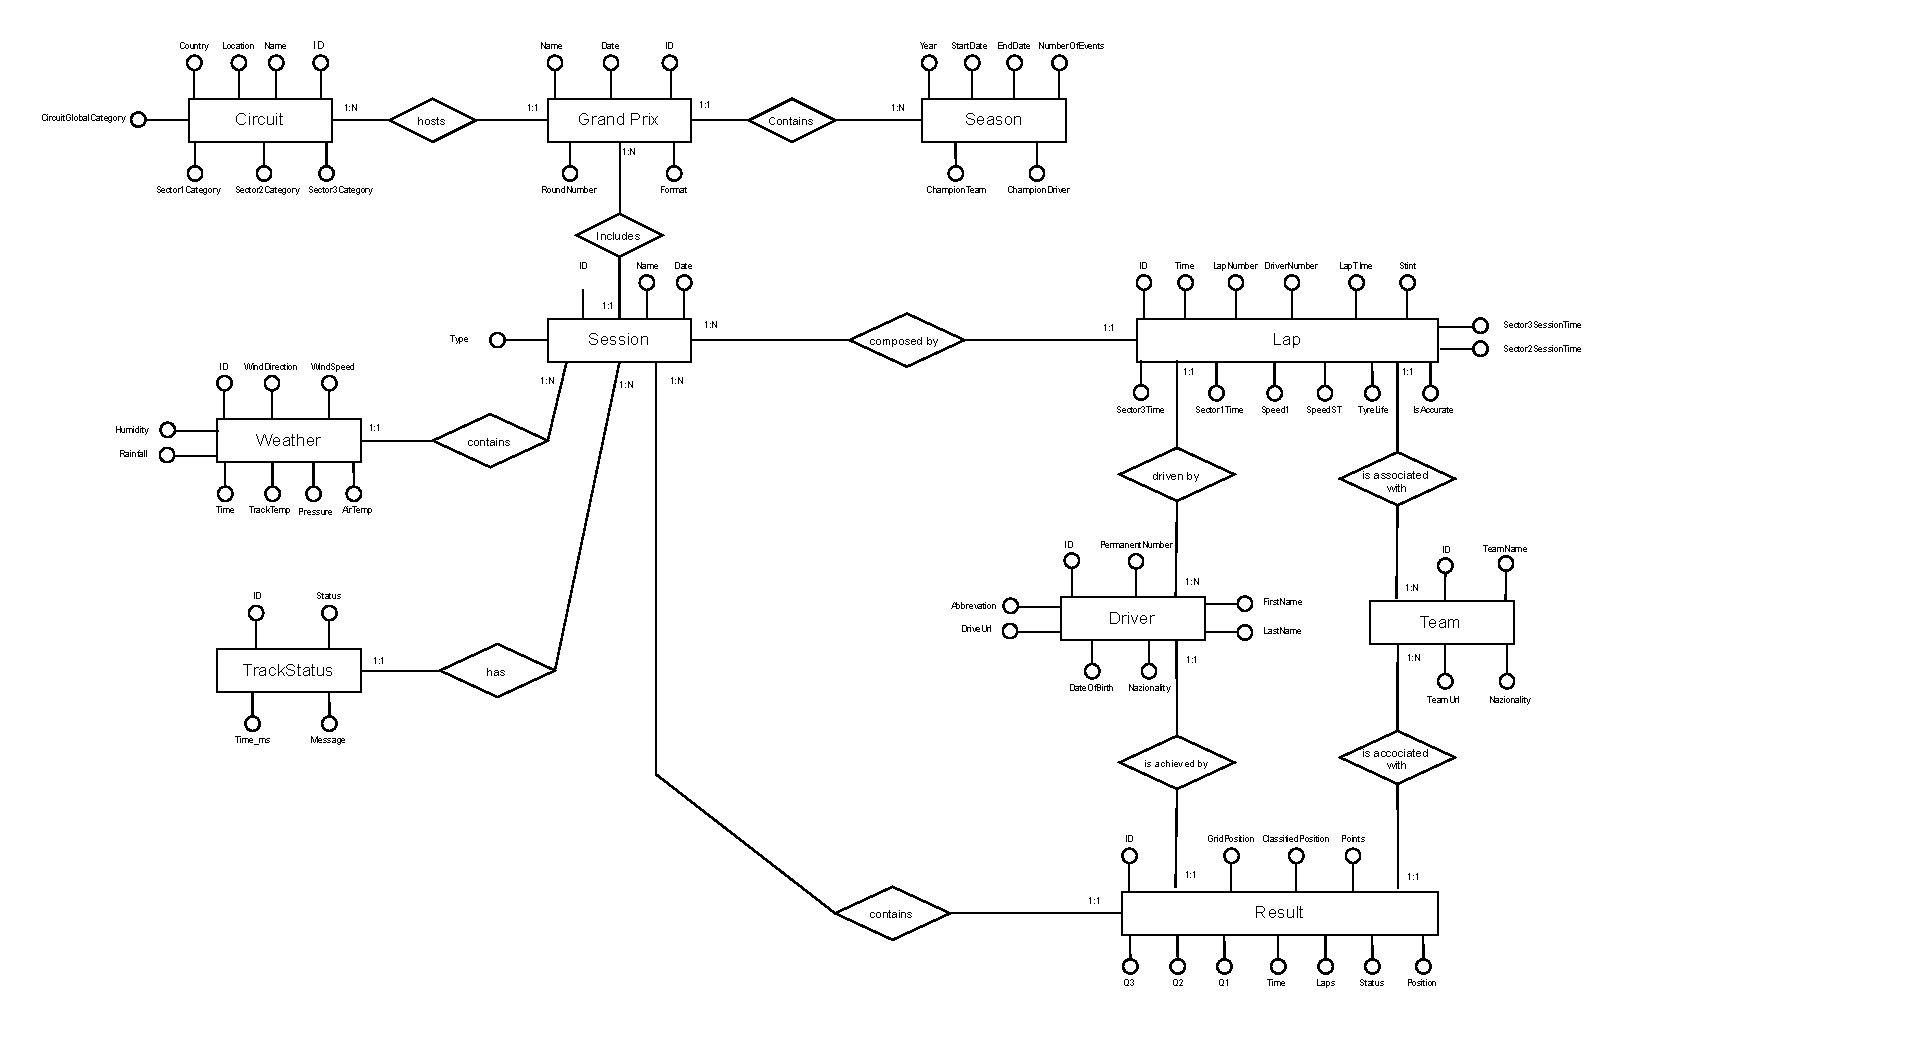
\includegraphics[width=0.90\textwidth]{image/e_r.pdf}
		\caption{Overall Data Quality Score by Table}
		\label{fig:dq-overall-score-by-table}
	\end{figure}
	
	% ------------------------------------------------------------
	\subsubsection{Data Quality Score by Dimension}
	% ------------------------------------------------------------
	
	This plot compares the quality dimensions across the whole database.
	It is useful to understand whether the main problem is completeness, uniqueness, validity, consistency, timeliness, accuracy, or referential integrity.
	
	\begin{figure}[H]
		\centering
		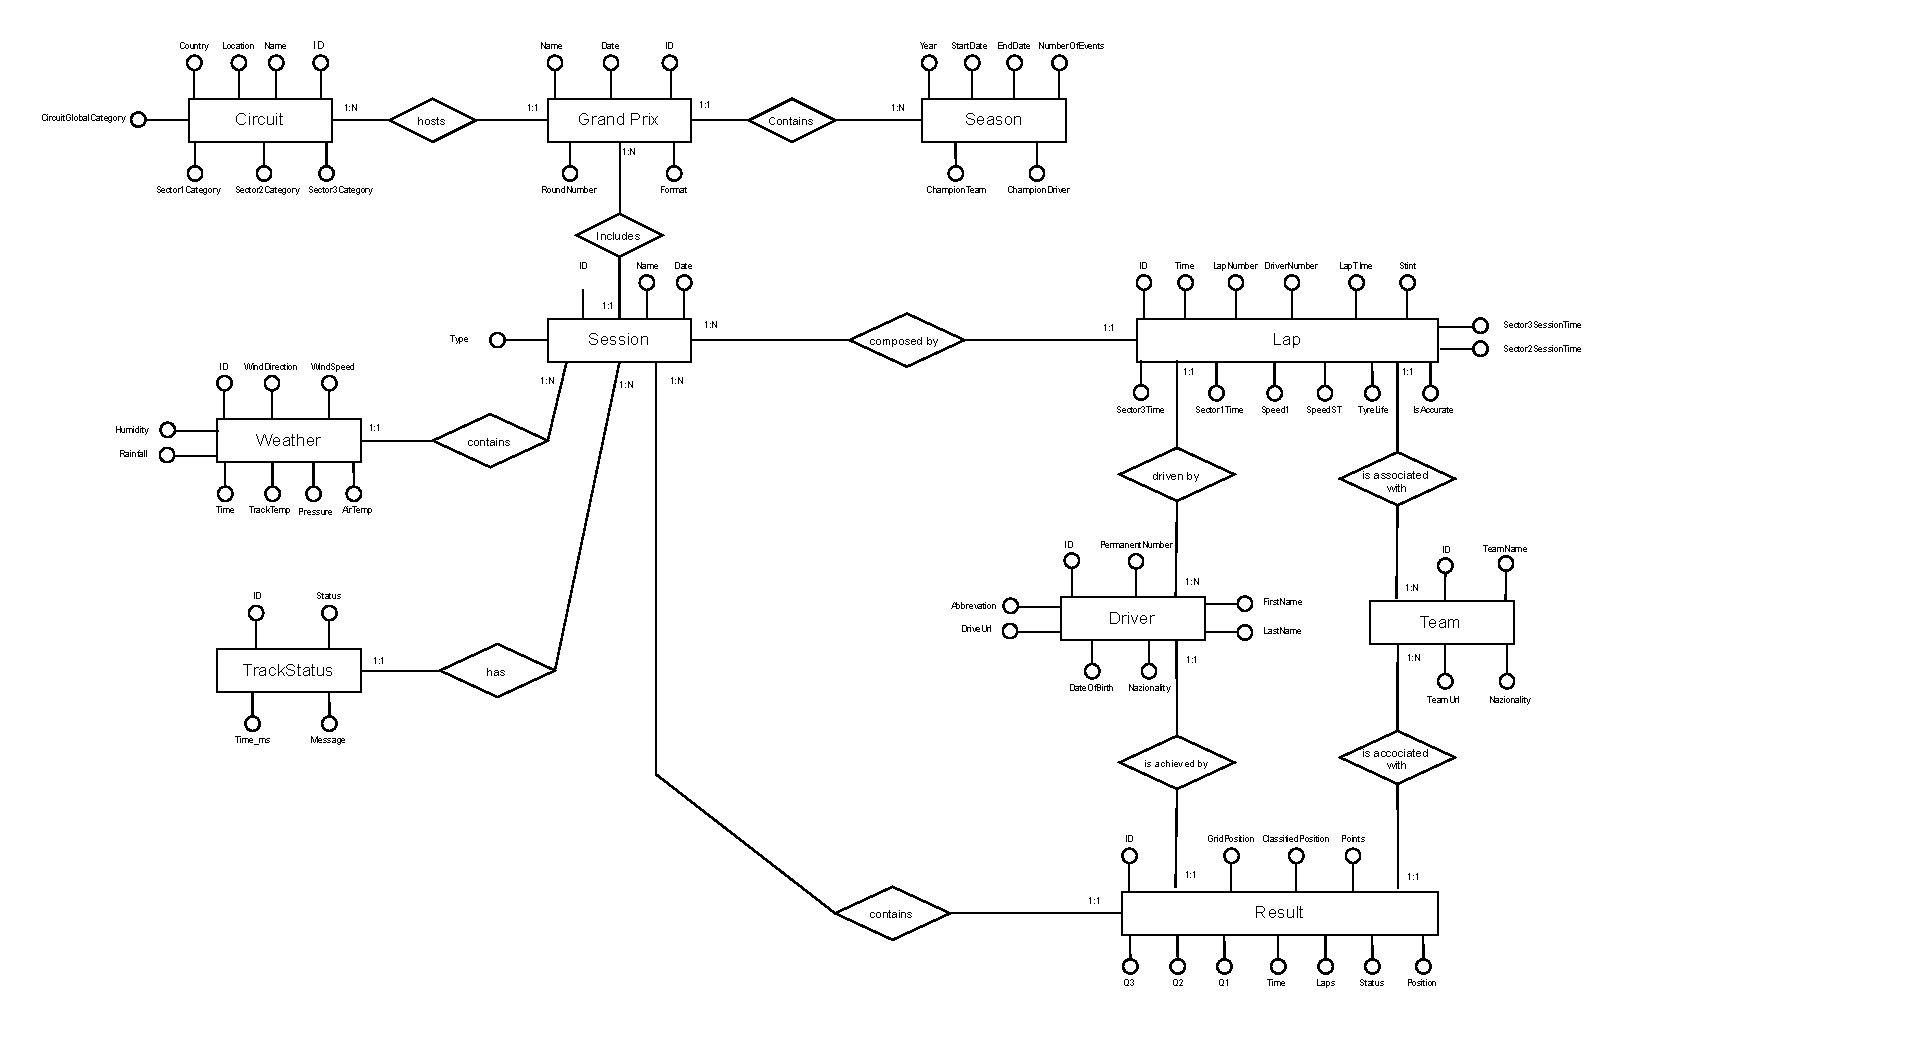
\includegraphics[width=0.90\textwidth]{image/e_r.pdf}
		\caption{Data Quality Score by Dimension}
		\label{fig:dq-score-by-dimension}
	\end{figure}
	
	% ------------------------------------------------------------
	\subsubsection{Heatmap of Table-Dimension Scores}
	% ------------------------------------------------------------
	
	A heatmap is useful to show which tables and dimensions have the weakest scores.
	This figure allows the reader to identify problematic combinations, such as low completeness in \texttt{lap} or low validity in \texttt{weather}.
	
	\begin{figure}[H]
		\centering
		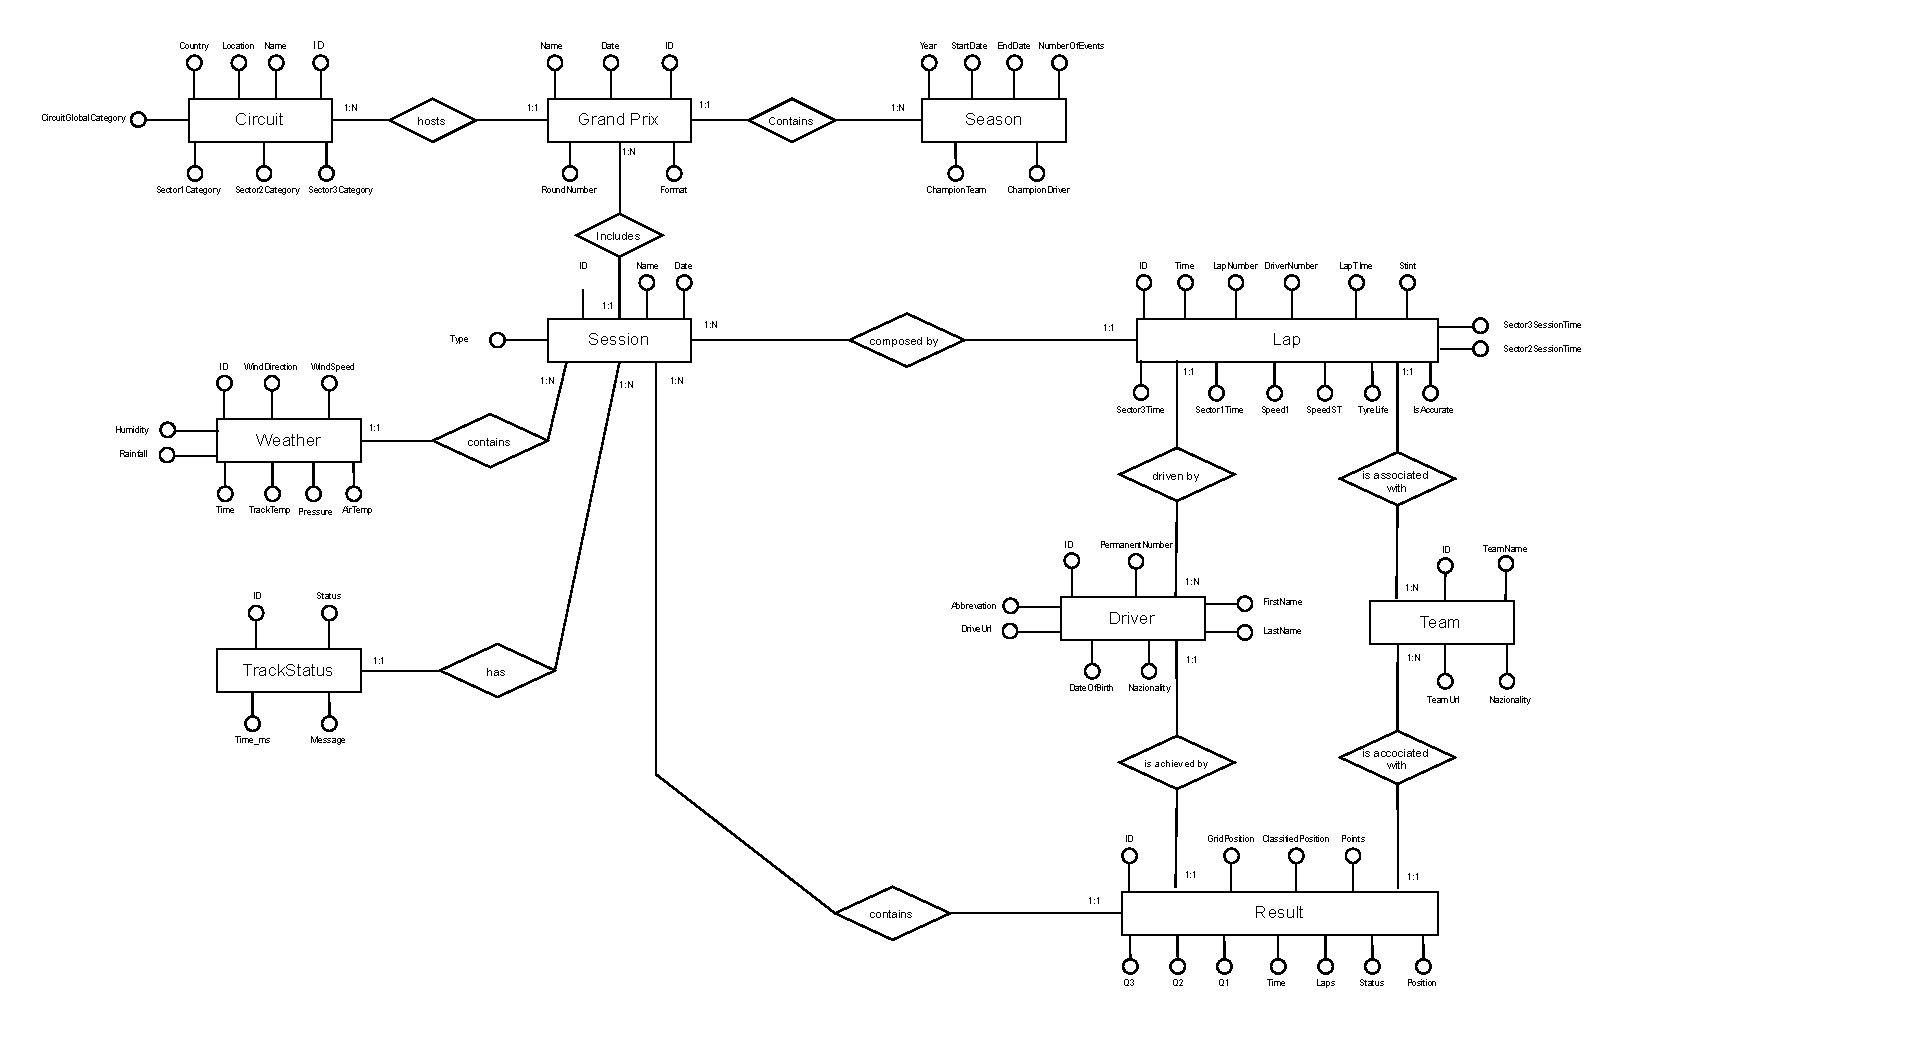
\includegraphics[width=0.90\textwidth]{image/e_r.pdf}
		\caption{Heatmap of Data Quality Scores by Table and Dimension}
		\label{fig:dq-score-heatmap}
	\end{figure}
	
	% ------------------------------------------------------------
	\subsubsection{Missing Values Summary}
	% ------------------------------------------------------------
	
	This plot summarizes missing values by table or by column.
	It supports the completeness analysis and helps identify attributes that require special attention during cleaning.
	
	\begin{figure}[H]
		\centering
		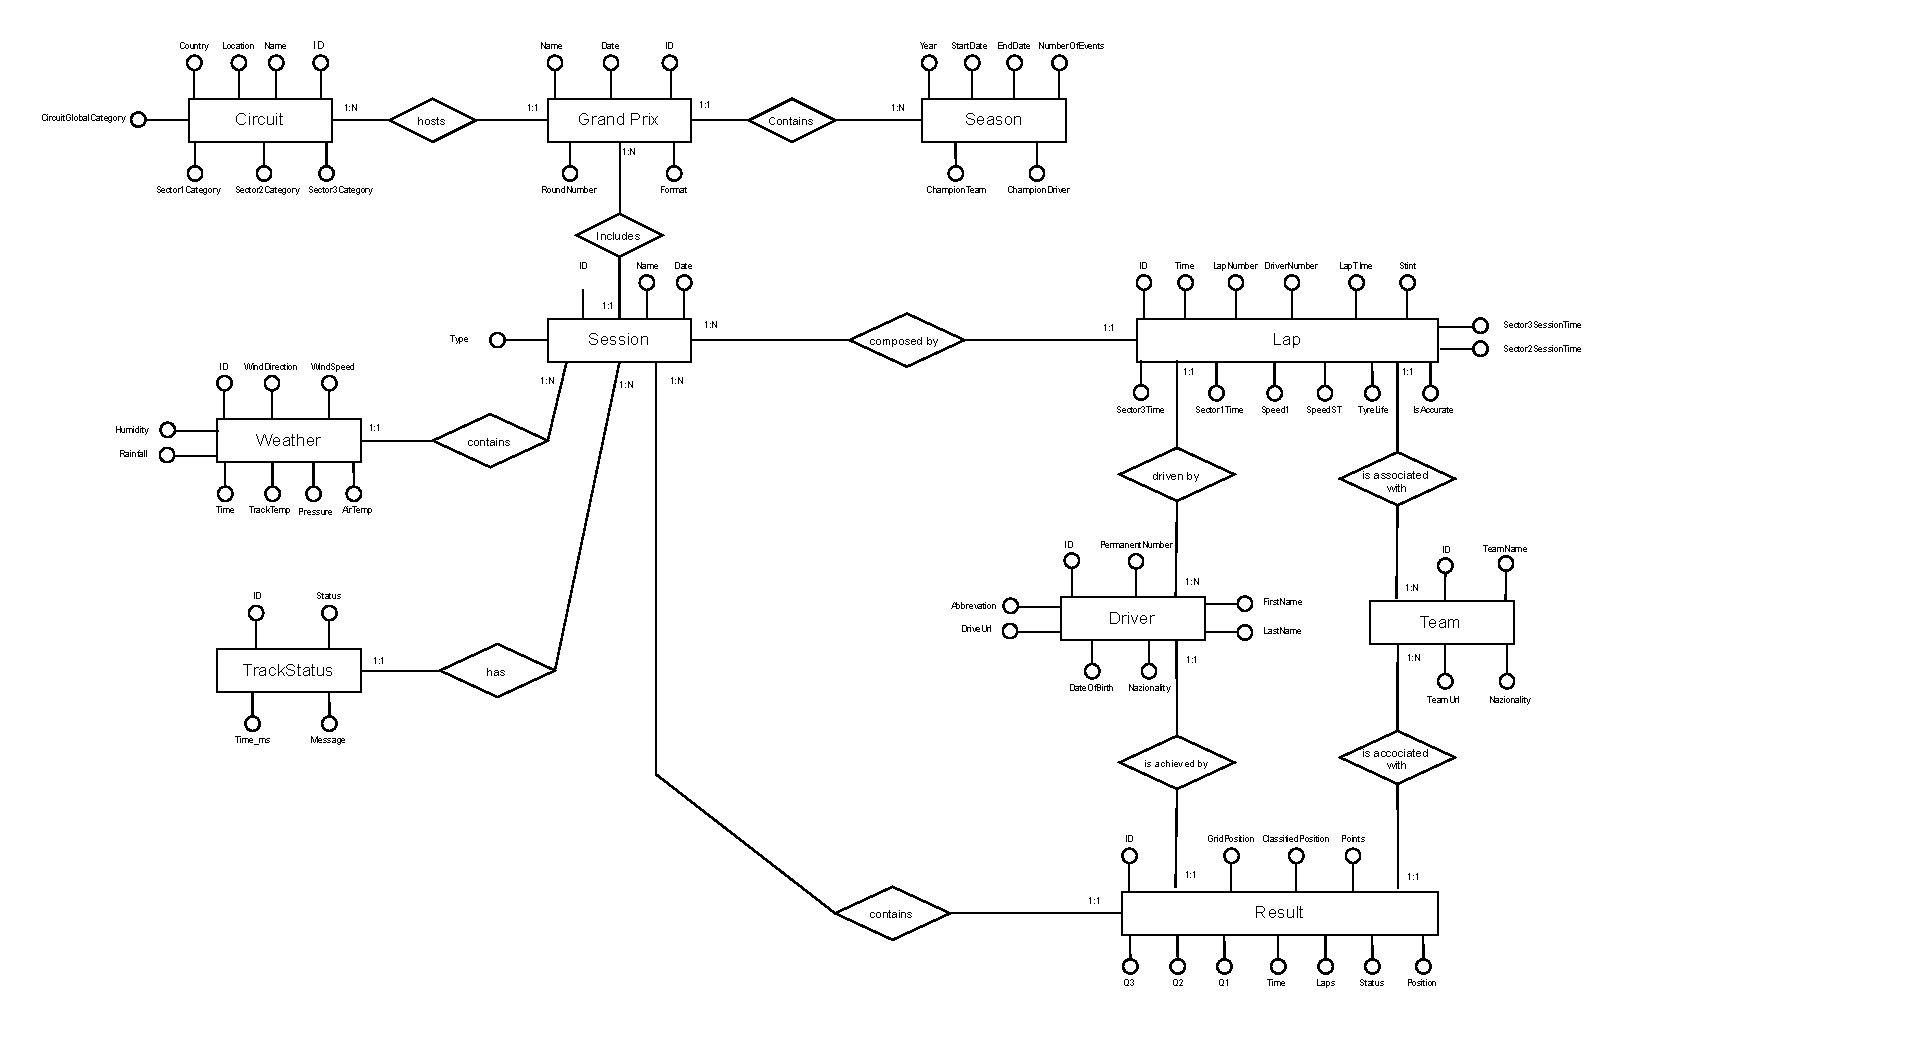
\includegraphics[width=0.90\textwidth]{image/e_r.pdf}
		\caption{Missing Values Summary}
		\label{fig:dq-missing-values-summary}
	\end{figure}
	
	% ------------------------------------------------------------
	\subsubsection{Referential Integrity Issues}
	% ------------------------------------------------------------
	
	This plot summarizes broken references between child and parent tables.
	It is especially important before applying explicit SQL foreign key constraints.
	
	\begin{figure}[H]
		\centering
		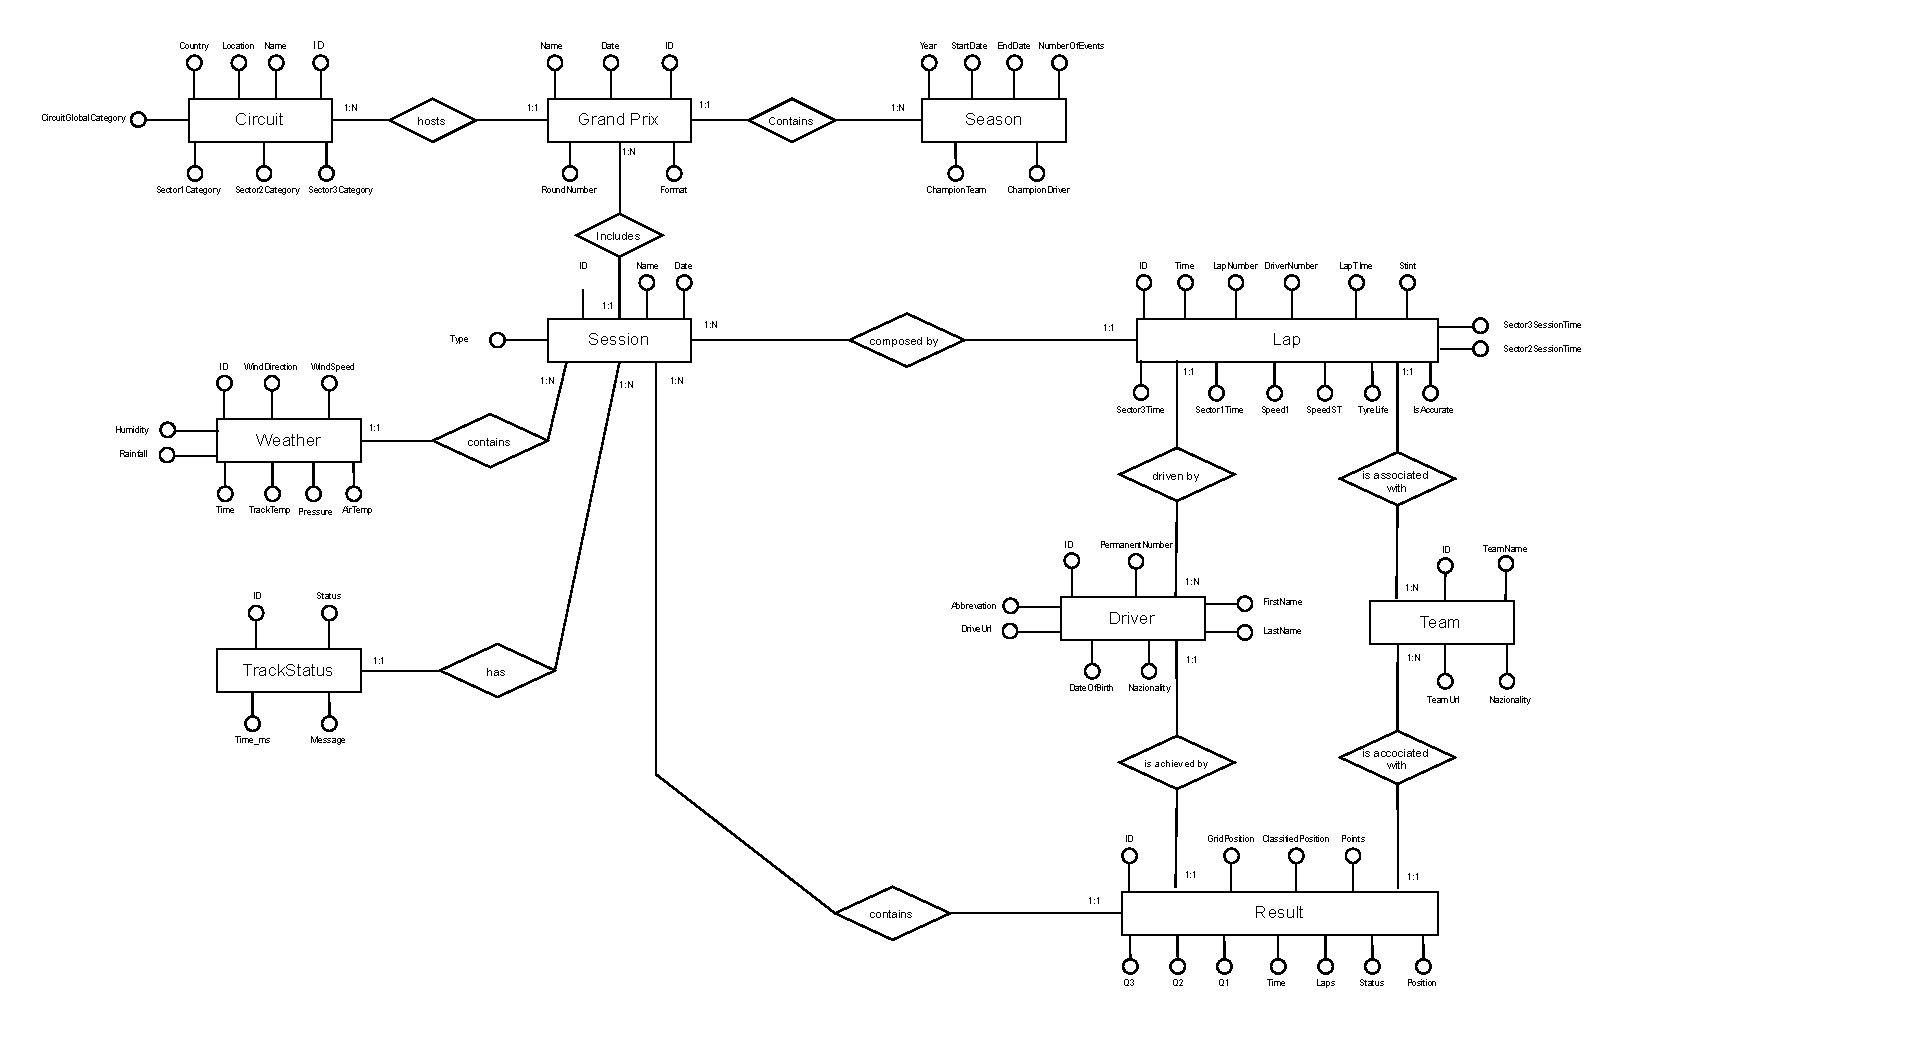
\includegraphics[width=0.90\textwidth]{image/e_r.pdf}
		\caption{Referential Integrity Issues by Relationship}
		\label{fig:dq-referential-integrity-issues}
	\end{figure}
	


	%============================================================
	\section{Focused Missing Values Analysis}
	%============================================================
	
	Missing values are treated as a focused data quality problem mainly related to the
	\textit{Completeness} dimension. However, in this project, not every null value is
	automatically considered a data quality error. Some attributes may be null because the
	information is not applicable in a specific Formula 1 context.
	
	For this reason, the missing values analysis does not simply count null values. It also
	classifies them according to their meaning in the domain.
	
	% ------------------------------------------------------------
	\subsection{Missing Values and Completeness}
	% ------------------------------------------------------------
	
	The first interpretation of missing values is connected to completeness. A table is
	complete when all required values are present. In this project, structural identifiers and
	foreign keys are considered mandatory, because they are necessary to connect the
	reconciled tables.
	
	Examples of structural attributes are:
	
	\begin{itemize}
		\item \texttt{session\_id}
		\item \texttt{driver\_id}
		\item \texttt{team\_id}
		\item \texttt{lap\_id}
		\item \texttt{result\_id}
	\end{itemize}
	
	If one of these attributes is missing, the row may become unusable for relational joins
	and for the later Data Warehouse loading phase.
	
	By contrast, some analytical attributes may be missing without immediately invalidating
	the row. For example, a missing \texttt{lap\_time\_ms} must be investigated, but it is not
	equivalent to a missing primary or foreign key.
	
	% ------------------------------------------------------------
	\subsection{MCAR, MAR, and MNAR Classification}
	% ------------------------------------------------------------
	
	The theoretical classification of missing values distinguishes between three main
	mechanisms: MCAR, MAR, and MNAR.
	
	\begin{longtable}{p{3cm}p{6cm}p{5.5cm}}
		\toprule
		\textbf{Mechanism} & \textbf{Meaning} & \textbf{Interpretation in this project} \\
		\midrule
		\endfirsthead
		
		\toprule
		\textbf{Mechanism} & \textbf{Meaning} & \textbf{Interpretation in this project} \\
		\midrule
		\endhead
		
		MCAR &
		Missing Completely At Random. The missingness has no relationship with other
		variables in the dataset. &
		Possible case for small random gaps in contextual data, such as occasional missing
		weather observations. \\
		\midrule
		
		MAR &
		Missing At Random. The missingness depends on other observed variables. &
		Possible case for qualifying times, where \texttt{q2\_ms} or \texttt{q3\_ms} may be missing
		depending on the driver's progression through the qualifying session. \\
		\midrule
		
		MNAR &
		Missing Not At Random. The missingness depends on the missing value itself or on an
		unobserved reason. &
		Possible suspicious case when missing lap times are related to problematic laps, deleted
		laps, inaccurate laps, or special racing conditions. \\
		\bottomrule
	\end{longtable}
	
	This classification is useful because different missing mechanisms require different
	cleaning strategies. In this project, missing values are not automatically imputed. Instead,
	they are first classified and then used to define motivated cleaning or filtering decisions.
	
	% ------------------------------------------------------------
	\subsection{Expected NULL Values}
	% ------------------------------------------------------------
	
	Some null values are expected and should not be interpreted as data quality errors. These
	values are null because the corresponding attribute is meaningful only under specific
	conditions.
	
	Examples include:
	
	\begin{longtable}{p{4cm}p{5cm}p{5.5cm}}
		\toprule
		\textbf{Attribute} & \textbf{Condition} & \textbf{Interpretation} \\
		\midrule
		\endfirsthead
		
		\toprule
		\textbf{Attribute} & \textbf{Condition} & \textbf{Interpretation} \\
		\midrule
		\endhead
		
		\texttt{q1\_ms}, \texttt{q2\_ms}, \texttt{q3\_ms} &
		Session type is Race &
		Expected null, because qualifying segment times are not applicable to race sessions. \\
		\midrule
		
		\texttt{q2\_ms} &
		Driver did not reach Q2 &
		Expected null, because the driver has no Q2 time. \\
		\midrule
		
		\texttt{q3\_ms} &
		Driver did not reach Q3 &
		Expected null, because the driver has no Q3 time. \\
		\midrule
		
		\texttt{pit\_in\_time\_ms} &
		Normal lap &
		Expected null, because the lap is not an in-lap. \\
		\midrule
		
		\texttt{pit\_out\_time\_ms} &
		Normal lap &
		Expected null, because the lap is not an out-lap. \\
		\midrule
		
		\texttt{deleted\_reason} &
		Lap is not deleted &
		Expected null, because no deletion reason exists. \\
		\bottomrule
	\end{longtable}
	
	Therefore, the missing values analysis must distinguish between expected nulls and real
	data quality problems.
	
	% ------------------------------------------------------------
	\subsection{Problematic NULL Values}
	% ------------------------------------------------------------
	
	A null value is considered problematic when it affects the identification, connection, or
	analytical usability of a row.
	
	Examples of problematic null values are:
	
	\begin{itemize}
		\item missing primary keys or surrogate identifiers;
		\item missing foreign keys required to join tables;
		\item missing \texttt{driver\_id} or \texttt{team\_id} in fact-like tables;
		\item missing \texttt{session\_id} in session-dependent tables;
		\item missing \texttt{lap\_number} in the lap table;
		\item missing \texttt{lap\_time\_ms} in laps that should represent valid timed laps.
	\end{itemize}
	
	These missing values are flagged by the assessment script and are later considered during
	the cleaning phase.
	
	The output of this analysis is expected to include:
	
	\begin{itemize}
		\item a summary of missing values by table;
		\item a summary of missing values by column;
		\item a classification of expected and problematic null values;
		\item a list of rows requiring further inspection.
	\end{itemize}


	
	% ============================================================
	\section{Focused Outlier Detection}
	% ============================================================
	
	Outlier detection is treated as a focused data quality analysis related mainly to
	\textit{Accuracy}, \textit{Validity}, and \textit{Consistency}. The goal is to identify
	values that are statistically unusual or suspicious from a domain perspective.
	
	In this project, an outlier is not automatically considered a wrong value. Formula 1 data
	can contain extreme but valid values due to pit stops, Safety Car periods, red flags,
	weather conditions, deleted laps, inaccurate laps, or other special racing situations.
	
	Therefore, outlier detection is used to flag suspicious records, not to automatically delete
	them.
	
	% ------------------------------------------------------------
	\subsection{IQR Method}
	% ------------------------------------------------------------
	
	The Interquartile Range method is a simple and interpretable univariate outlier detection
	technique. It is based on the first quartile, the third quartile, and the interquartile range.
	
	\[
	IQR = Q3 - Q1
	\]
	
	A value is considered suspicious if it falls outside the following interval:
	
	\[
	LowerBound = Q1 - k \cdot IQR
	\]
	
	\[
	UpperBound = Q3 + k \cdot IQR
	\]
	
	where \(k\) is usually set to 1.5 for standard outlier detection or to a larger value for a
	more conservative analysis.
	
	In this project, the IQR method can be applied to numerical attributes such as:
	
	\begin{itemize}
		\item \texttt{lap\_time\_ms}
		\item \texttt{sector1\_time\_ms}
		\item \texttt{sector2\_time\_ms}
		\item \texttt{sector3\_time\_ms}
		\item speed attributes
		\item weather attributes
	\end{itemize}
	
	% ------------------------------------------------------------
	\subsection{Modified Z-score}
	% ------------------------------------------------------------
	
	The Modified Z-score is a robust alternative to the classical Z-score. It uses the median
	and the Median Absolute Deviation instead of the mean and standard deviation.
	
	\[
	M_i = \frac{0.6745(x_i - median(x))}{MAD}
	\]
	
	where:
	
	\[
	MAD = median(|x_i - median(x)|)
	\]
	
	A value is usually considered suspicious when:
	
	\[
	|M_i| > 3.5
	\]
	
	This method is useful because Formula 1 performance data may be skewed. For example,
	lap times may include normal fast laps, slow laps, pit laps, laps under Safety Car, and
	other special cases. Using the median makes the method less sensitive to extreme values.
	
	% ------------------------------------------------------------
	\subsection{Consensus and Multi-method Flag}
	% ------------------------------------------------------------
	
	No single outlier detection method is perfect. For this reason, the assessment uses a
	simple consensus strategy.
	
	Each numerical value can be flagged by one or more methods. The number of methods
	that flag the same value is used as an indicator of anomaly strength.
	
	\begin{longtable}{p{3cm}p{5cm}p{6cm}}
		\toprule
		\textbf{Number of Flags} & \textbf{Interpretation} & \textbf{Action} \\
		\midrule
		\endfirsthead
		
		\toprule
		\textbf{Number of Flags} & \textbf{Interpretation} & \textbf{Action} \\
		\midrule
		\endhead
		
		0 &
		Normal value &
		No action required. \\
		\midrule
		
		1 &
		Weak anomaly &
		Review only if the attribute is important for the analysis. \\
		\midrule
		
		2 or more &
		Stronger suspicious value &
		Investigate before using the row in the Data Warehouse. \\
		\bottomrule
	\end{longtable}
	
	In the first implementation, the consensus is based on the IQR method and the Modified
	Z-score. More advanced techniques, such as Isolation Forest or Local Outlier Factor, can
	be added later if necessary.
	
	% ------------------------------------------------------------
	\subsection{Domain Interpretation}
	% ------------------------------------------------------------
	
	The statistical detection of an outlier is not sufficient to decide whether a record must be
	removed or corrected. Each suspicious value must be interpreted in the Formula 1 domain.
	
	For example, a very slow lap can be caused by:
	
	\begin{itemize}
		\item an in-lap;
		\item an out-lap;
		\item a pit stop;
		\item a Safety Car period;
		\item a Virtual Safety Car period;
		\item rain or wet track conditions;
		\item red flags or yellow flags;
		\item an inaccurate or deleted lap.
	\end{itemize}
	
	For this reason, the output of the outlier detection script is used as input for later
	cleaning and analytical filtering decisions. The script does not delete outliers
	automatically. It only flags them and provides evidence for manual or rule-based
	interpretation.
	
	The expected outputs are:
	
	\begin{itemize}
		\item an outlier summary by table and column;
		\item row-level outlier flags;
		\item a consensus score for suspicious values;
		\item plots showing outlier distributions;
		\item a list of records requiring further review.
	\end{itemize}



	% ============================================================
	\section{Optional LLM Support}
	% ============================================================
	
	A Large Language Model can be used as an optional support layer for interpreting the
	Data Quality Assessment outputs. However, it is not part of the deterministic data quality
	pipeline and it does not replace the Python-based checks.
	
	The official assessment results are produced only by deterministic scripts. These scripts
	compute quality scores, detect missing values, identify outliers, and generate row-level
	issue files. The LLM can only be used after these outputs have been generated.
	
	% ------------------------------------------------------------
	\subsection{Not Part of the Deterministic Pipeline}
	% ------------------------------------------------------------
	
	The LLM is not used to decide whether a value is valid, whether a row must be removed,
	or whether a cleaning rule must be applied.
	
	The deterministic part of the pipeline includes:
	
	\begin{itemize}
		\item general data quality checks;
		\item missing values analysis;
		\item outlier detection;
		\item referential integrity checks;
		\item row-level flags;
		\item scorecard generation.
	\end{itemize}
	
	These steps are reproducible because the same input data and the same rules always
	produce the same outputs.
	
	By contrast, LLM outputs are probabilistic and may vary depending on the prompt, model,
	and configuration. For this reason, the LLM is separated from the official assessment
	logic.
	
	% ------------------------------------------------------------
	\subsection{Used Only for Explanation}
	% ------------------------------------------------------------
	
	If used, the LLM receives only aggregated and already generated outputs, such as:
	
	\begin{itemize}
		\item data quality scorecards;
		\item missing value summaries;
		\item missing value classifications;
		\item outlier summaries;
		\item referential integrity issue summaries.
	\end{itemize}
	
	The goal is to generate a natural-language explanation of the results. Possible outputs
	include:
	
	\begin{itemize}
		\item a stakeholder-oriented data quality summary;
		\item a technical explanation of the main quality problems;
		\item a draft paragraph for the final report;
		\item a preliminary list of cleaning priorities.
	\end{itemize}
	
	The LLM does not access the PostgreSQL database directly and does not modify any data.
	
	% ------------------------------------------------------------
	\subsection{Manually Validated Output}
	% ------------------------------------------------------------
	
	Every LLM-generated output must be manually reviewed before being included in the
	project documentation.
	
	The LLM output is treated as a draft, not as an authoritative result. The final explanation
	included in the report must be checked against the original scorecards and issue files.
	
	For transparency, the following files can be stored:
	
	\begin{itemize}
		\item \texttt{llm\_input\_dqa\_summary.json}
		\item \texttt{llm\_prompt\_dqa\_interpretation.txt}
		\item \texttt{llm\_output\_dqa\_interpretation.md}
		\item \texttt{llm\_human\_review\_notes.md}
	\end{itemize}
	
	This makes the use of the LLM explicit, controlled, and auditable.
	
	In summary, the LLM is used only as an explanatory assistant. The official data quality
	decisions remain based on deterministic and reproducible checks.
	% =======================================================
	\section{Conclusion}
	% =======================================================
	

	The final goal is not only to detect problems, but also to produce evidence for the next phase.
	The generated scorecards, issue files, and plots will guide the cleaning script and will support the documentation of all data quality decisions in the final project report.
	
\end{document}
